\documentclass[12pt,a4paper]{article}
\usepackage[utf8]{inputenc}
\usepackage{graphicx}
\usepackage{booktabs}
\usepackage{amsmath}
\usepackage{hyperref}
\usepackage{geometry}
\usepackage{float}

\geometry{margin=1in}

\title{%
  \textbf{P15: Sentiment Classification of IMDb Movie Reviews}\\
  \vspace{0.5em}
  \large CS485 -- Project Report
}
\author{%
  Zervos Spiridon Chrisovalantis (csd4878) \\
  Drakakis Rafail (csd5310)
}
\date{\today}

\begin{document}

\maketitle
\thispagestyle{empty}

\begin{abstract}
  We present an end-to-end pipeline for sentiment classification of the IMDb Movie Reviews dataset using both classical and deep learning techniques. We preprocess the data, extract features, train multiple models, and evaluate their performance. Classical ML models include Logistic Regression, Naive Bayes, and Linear SVM trained on TF–IDF vectors. Deep learning models include LSTM and 1D-CNN built using PyTorch with learned embeddings. We analyze accuracy, confusion matrices, and inference time. Our results show strong performance from classical methods, competitive CNN results, and poor LSTM learning without pretrained embeddings or tuning.
\end{abstract}

\newpage
\tableofcontents
\newpage

\section{Introduction}
Sentiment analysis seeks to classify text into categories such as positive or negative sentiment. The IMDb dataset offers a widely used benchmark of 50,000 labeled movie reviews. We compare two families of sentiment classification models:
\begin{itemize}
  \item \textbf{Classical ML}: Feature engineering with TF–IDF followed by Logistic Regression, Naive Bayes, and Linear SVM.
  \item \textbf{Deep Learning}: LSTM and CNN architectures with learned word embeddings and end-to-end training in PyTorch.
\end{itemize}

\section{Dataset}
\begin{itemize}
  \item \textbf{Name:} IMDb Large Movie Review Dataset
  \item \textbf{Size:} 25,000 training and 25,000 test samples
  \item \textbf{Labels:} Binary sentiment – Positive (1), Negative (0)
  \item \textbf{Source:} \url{https://ai.stanford.edu/~amaas/data/sentiment/}
\end{itemize}

\section{Preprocessing}
\begin{itemize}
  \item Downloaded and extracted from Google Drive.
  \item Text normalization: lowercasing, tokenization (using NLTK \texttt{word\_tokenize}), removal of punctuation, numbers, and stopwords.
  \item For deep models: vocabulary built with a minimum frequency of 2 and capped at 20,000 tokens. Input sequences are padded or truncated to a maximum length of 200.
\end{itemize}

\section{Feature Engineering}
\begin{itemize}
  \item \textbf{Classical ML:} TF–IDF vectorization with unigrams and 5,000 max features.
  \item \textbf{Deep Learning:} Trainable embedding layers of dimension 100.
\end{itemize}

\section{Model Architectures \& Training Details}
\subsection{Classical Models}
\begin{description}
  \item[Logistic Regression:] $\ell_2$ regularization, $C = 1.0$, max\_iter = 1000
  \item[Multinomial Naive Bayes:] $\alpha = 1.0$
  \item[Linear SVM:] $C = 1.0$
\end{description}

\subsection{Deep Learning Models}
\begin{itemize}
  \item \textbf{Embedding Layer:} Embedding dimension = 100
  \item \textbf{LSTM:} Single-layer LSTM with 128 hidden units; classifier uses final hidden state
  \item \textbf{CNN:} 1D convolutions with filter sizes [3, 4, 5], 100 filters each; followed by max pooling and a fully connected layer
  \item \textbf{Training:} Optimized with Adam, learning rate = $1e^{-3}$, 5 epochs, batch size = 64
\end{itemize}

\section{Results}
\subsection{Classical Machine Learning}

\begin{table}[H]
  \centering
  \caption{Accuracy and Inference Time (ms/sample) on 25,000 test samples}
  \label{tab:classical-summary}
  \begin{tabular}{lcc}
    \toprule
    \textbf{Model}          & \textbf{Accuracy} & \textbf{Time (ms/sample)} \\
    \midrule
    Logistic Regression     & 0.880             & 0.47                     \\
    Multinomial Naïve Bayes & 0.840             & 0.13                     \\
    Linear SVM              & 0.863             & 0.65                     \\
    \bottomrule
  \end{tabular}
\end{table}

\begin{table}[H]
  \centering
  \caption{Classification Report for Logistic Regression}
  \begin{tabular}{lcccc}
    \toprule
    \textbf{Class} & \textbf{Precision} & \textbf{Recall} & \textbf{F1-score} & \textbf{Support} \\
    \midrule
    Negative & 0.88 & 0.88 & 0.88 & 12500 \\
    Positive & 0.88 & 0.88 & 0.88 & 12500 \\
    \midrule
    \multicolumn{5}{l}{\textbf{Overall accuracy:} 0.88} \\
    \bottomrule
  \end{tabular}
\end{table}

\begin{figure}[H]
  \centering
  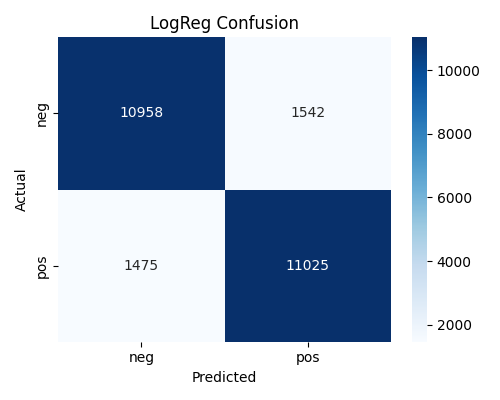
\includegraphics[width=0.6\textwidth]{figures/LogReg_confusion.png}
  \caption{Confusion matrix for Logistic Regression}
\end{figure}

\begin{figure}[H]
  \centering
  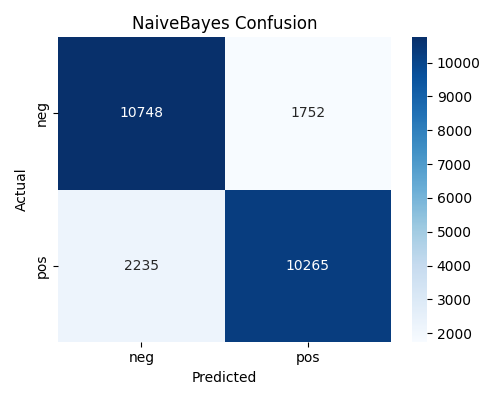
\includegraphics[width=0.45\textwidth]{figures/NaiveBayes_confusion.png}
  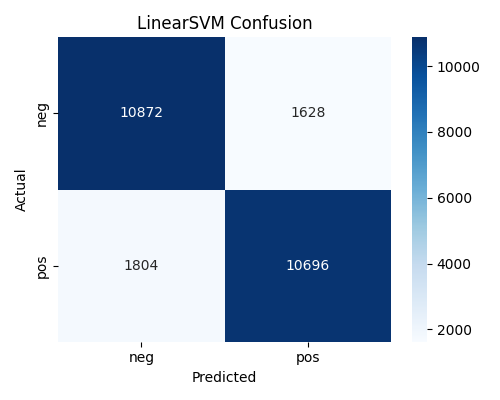
\includegraphics[width=0.45\textwidth]{figures/LinearSVM_confusion.png}
  \caption{Confusion matrices: Naïve Bayes (left), Linear SVM (right)}
\end{figure}

\subsection{Deep Learning}

\begin{table}[H]
  \centering
  \caption{Test Accuracy for Deep Models}
  \label{tab:dl-results}
  \begin{tabular}{lcc}
    \toprule
    \textbf{Model} & \textbf{Accuracy} & \textbf{Notes} \\
    \midrule
    LSTM & 0.511 & Underfitting, poor learning across epochs \\
    CNN  & 0.856 & Competitive with classical models \\
    \bottomrule
  \end{tabular}
\end{table}

\begin{figure}[H]
  \centering
  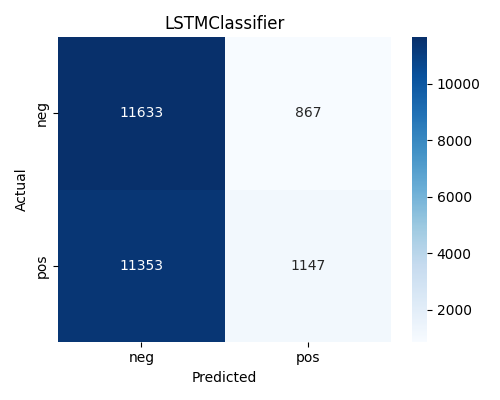
\includegraphics[width=0.45\textwidth]{figures/LSTMClassifier_confusion.png}
  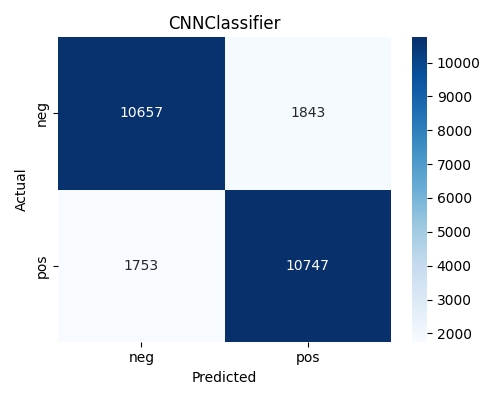
\includegraphics[width=0.45\textwidth]{figures/CNNClassifier_confusion.png}
  \caption{Confusion matrices: LSTM (left), CNN (right)}
\end{figure}

\section{Discussion}
\begin{itemize}
  \item \textbf{Inference speed:} Naïve Bayes is fastest (0.13ms/sample), followed by Logistic Regression (0.47ms), and Linear SVM (0.65ms).
  \item \textbf{Accuracy:} Logistic Regression is best overall (0.88), CNN comes close (0.856), and LSTM performs poorly (0.511).
  \item \textbf{Deep Learning Issues:}
    \begin{itemize}
      \item LSTM struggles due to lack of pretraining, insufficient data augmentation, and shallow architecture.
      \item CNN benefits from local n-gram pattern detection via convolution and max pooling.
    \end{itemize}
  \item \textbf{Generalization:} CNN is more robust than LSTM but needs GPU for fast training.
  \item \textbf{Short reviews:} Posed challenges for all models, especially with sarcasm or implicit sentiment.
\end{itemize}

\section{Conclusion}
We implemented a full classification pipeline using classical and deep learning models for sentiment analysis on the IMDb dataset. Classical methods with TF–IDF and Logistic Regression remain strong baselines for accuracy and speed. While the CNN shows promising results, the LSTM architecture underperformed due to training instability and lack of optimization. Further improvements may include hyperparameter tuning, pretrained embeddings, and attention mechanisms.

\end{document}
